%\documentclass[hyperref={pdfpagelabels=false},slidetop,9pt]{beamer}
\documentclass[slidetop,8pt]{beamer}
\usepackage[T1]{fontenc}
\usepackage[utf8]{inputenc}
\newcommand{\id}{71}
\newcommand{\nom}{Théorie des mécanismes}
\newcommand{\sequence}{04}
\newcommand{\nomsequence}{Liaisons entre les solides}
\newcommand{\num}{02}
\newcommand{\type}{KH}
\newcommand{\descrip}{Liaisons équivalentes, hyperstatisme, liaisons en série et en parallèle, théorie des graphes}
\newcommand{\competences}{B2-12: Proposer une modélisation des liaisons avec leurs caractéristiques géométriques. \\ &  B2-13: Proposer un modèle cinématique paramétré à partir d'un système réel, d'une maquette numérique ou d'u \\ &  B2-17: Simplifier un modèle de mécanisme. \\ &  B2-18: Modifier un modèle pour le rendre isostatique. \\ &  C1-04: Proposer une démarche permettant d'obtenir une loi entrée-sortie géométrique.  \\ &  C2-05: Caractériser le mouvement d'un repère par rapport à un autre repère. \\ &  C2-06: Déterminer les relations entre les grandeurs géométriques ou cinématiques. }
\newcommand{\nbcomp}{7}
\newcommand{\systemes}{}
\newcommand{\systemesnum}{}
\newcommand{\systemessansaccent}{}
\newcommand{\ilot}{2}
\newcommand{\ilotstr}{02}
\newcommand{\dossierilot}{\detokenize{Ilot_02 }}

\usepackage{etex}
\usepackage{tikz}
\usepackage[european]{circuitikz}
\usepackage{pgf}
\usepackage[all]{xy}
\usepackage{pgfpages}
\usepackage{graphbox}
\usepackage{pdfpages}
%\usepackage[adobe-utopia]{mathdesign}
\usepackage{ifthen}
\usepackage{cancel}
\usepackage{framed}
\usepackage{subfig}
\usepackage{tabularx}
\usepackage{setspace}
\usepackage{soul}
\usepackage{schemabloc}
\usepackage{eqnarray}
\usepackage[dot, phantomtext]{dashundergaps}
\usepackage{media9}
\usepackage{multimedia}
\usepackage{textcomp}
\usefonttheme[onlymath]{serif}

\author{Renaud Costadoat}
\institute{Lycée Dorian}

\usepackage{multido}
\usepackage{multirow}
\usepackage{multicol} % Portions de texte en colonnes
\usepackage{flafter}%floatants après la référence

\usepackage{color}
\usepackage{xcolor}
\usepackage{colortbl}

\usepackage[gen]{eurosym}
\usepackage{tikz}
%\usepackage{pstricks,pst-node,pst-tree,pst-solides3d}
\usepackage{lmodern}
\usepackage[francais]{babel}
\usepackage{pslatex}
\usetheme{renaud}
\usepackage{times}
\usepackage[frenchmath]{newtxsf} % for sans serif symbols
\renewcommand{\familydefault}{\sfdefault}
%\usepackage{amsfonts}
%\usepackage{amsmath}
%\usepackage{mathastext}
\usepackage{verbatim}
\usepackage{moreverb}
%\usetikzlibrary{arrows,shapes}
\usepackage{graphicx}
\usepackage{psfrag}
\usepackage{wrapfig}
\usepackage{etoolbox}

\definecolor{gris25}{gray}{0.75}
\definecolor{bleu}{RGB}{18,33,98}
\definecolor{bleuf}{RGB}{42,94,171}
\definecolor{bleuc}{RGB}{231,239,247}
\definecolor{rougef}{RGB}{185,18,27}
\definecolor{rougec}{RGB}{255,188,204}%255,230,231
\definecolor{vertf}{RGB}{103,126,82}
\definecolor{vertc}{RGB}{220,255,191}

\setlength\parindent{24pt}
\parskip 7.2pt
\parindent 8pt

\newenvironment{rem}[1][\hsize]%
{%
    \def\FrameCommand
   {%
\rotatebox{90}{\textit{\textsf{Remarque}}} 
       {\color{bleuf}\vrule width 3pt}%
       \hspace{0pt}%must no space.
       \fboxsep=\FrameSep\colorbox{bleuc}%
  }%
    \MakeFramed{\hsize#1\advance\hsize-\width\FrameRestore}%
}%
{\endMakeFramed}%


\newenvironment{savoir}[1][\hsize]%
{%
    \def\FrameCommand
    {%
\rotatebox{90}{\textit{\textsf{Savoir}}} 
        {\color{bleuf}\vrule width 3pt}%
        \hspace{0pt}%must no space.
        \fboxsep=\FrameSep\colorbox{bleuc}%
    }%
    \MakeFramed{\hsize#1\advance\hsize-\width\FrameRestore}%
}%
{\endMakeFramed}%

\newenvironment{prob}[1][\hsize]%
{%
    \def\FrameCommand%
    {%
\rotatebox{90}{\textit{\textsf{Problematique}}} 
        {\color{rougef}\vrule width 3pt}%
        \hspace{0pt}%must no space.
        \fboxsep=\FrameSep\colorbox{rougec}%
    }%
    \MakeFramed{\hsize#1\advance\hsize-\width\FrameRestore}%
}%
{\endMakeFramed}%

\newenvironment{obj}[1][\hsize]%
{%
    \def\FrameCommand%
    {%
\rotatebox{90}{\textit{\textsf{Objectif}}} 
        {\color{vertf}\vrule width 3pt}%
        \hspace{0pt}%must no space.
        \fboxsep=\FrameSep\colorbox{vertc}%
    }%
    \MakeFramed{\hsize#1\advance\hsize-\width\FrameRestore}%
}%
{\endMakeFramed}%

\newenvironment{defi}[1][\hsize]%
{%
    \def\FrameCommand%
    {%
\rotatebox{90}{\textit{\textsf{Definition}}} 
        {\color{bleuf}\vrule width 3pt}%
        \hspace{0pt}%must no space.
        \fboxsep=\FrameSep\colorbox{rougec}%
    }%
    \MakeFramed{\hsize#1\advance\hsize-\width\FrameRestore}%
}%
{\endMakeFramed}%


\newenvironment{hypo}[1][\hsize]%
{%
    \def\FrameCommand%
    {%
\rotatebox{90}{\textit{\textsf{Hypothèse\\}}} 
        {\color{bleuf}\vrule width 3pt}%
        \hspace{0pt}%must no space.
        \fboxsep=\FrameSep\colorbox{bleuc}%
    }%
    \MakeFramed{\hsize#1\advance\hsize-\width\FrameRestore}%
}%
{\endMakeFramed}%


\newenvironment{prop}[1][\hsize]%
{%
    \def\FrameCommand%
    {%
\rotatebox{90}{\textit{\textsf{Propriété}}} 
        {\color{bleuf}\vrule width 3pt}%
        \hspace{0pt}%must no space.
        \fboxsep=\FrameSep\colorbox{bleuc}%
    }%
    \MakeFramed{\hsize#1\advance\hsize-\width\FrameRestore}%
}%
{\endMakeFramed}%

\newenvironment{props}[1][\hsize]%
{%
    \def\FrameCommand%
    {%
\rotatebox{90}{\textit{\textsf{Propriétés}}} 
        {\color{bleuf}\vrule width 3pt}%
        \hspace{0pt}%must no space.
        \fboxsep=\FrameSep\colorbox{bleuc}%
    }%
    \MakeFramed{\hsize#1\advance\hsize-\width\FrameRestore}%
}%
{\endMakeFramed}%

\newenvironment{exemple}[1][\hsize]%
{%
    \def\FrameCommand%
    {%
\rotatebox{90}{\textit{\textsf{Exemple}}} 
        {\color{vertf}\vrule width 3pt}%
        \hspace{0pt}%must no space.
        \fboxsep=\FrameSep\colorbox{vertc}%
    }%
    \MakeFramed{\hsize#1\advance\hsize-\width\FrameRestore}%
}%
{\endMakeFramed}%

\newenvironment{resultat}[1][\hsize]%
{%
    \def\FrameCommand%
    {%
\rotatebox{90}{\textit{\textsf{Résultat}}} 
        {\color{rougef}\vrule width 3pt}%
%        {\color{bleuf}\vrule width 3pt}%
        \hspace{0pt}%must no space.
        \fboxsep=\FrameSep\colorbox{rougec}%
    }%
    \MakeFramed{\hsize#1\advance\hsize-\width\FrameRestore}%
}%
{\endMakeFramed}%

\newenvironment{methode}[1][\hsize]%
{%
    \def\FrameCommand%
    {%
\rotatebox{90}{\textit{\textsf{Méthode\\}}} 
        {\color{rougef}\vrule width 3pt}%
        \hspace{0pt}%must no space.
        \fboxsep=\FrameSep\colorbox{rougec}%
    }%
    \MakeFramed{\hsize#1\advance\hsize-\width\FrameRestore}%
}%
{\endMakeFramed}%

\newenvironment{theo}[1][\hsize]%
{%
    \def\FrameCommand%
    {%
\rotatebox{90}{\textit{\textsf{Théorème\\}}} 
        {\color{rougef}\vrule width 3pt}%
        \hspace{0pt}%must no space.
        \fboxsep=\FrameSep\colorbox{rougec}%
    }%
    \MakeFramed{\hsize#1\advance\hsize-\width\FrameRestore}%
}%
{\endMakeFramed}%

\newenvironment{warn}[1][\hsize]%
{%
    \def\FrameCommand%
    {%
\rotatebox{90}{\textit{\textsf{Attention\\}}} 
        {\color{rougef}\vrule width 3pt}%
        \hspace{0pt}%must no space.
        \fboxsep=\FrameSep\colorbox{rougec}%
    }%
    \MakeFramed{\hsize#1\advance\hsize-\width\FrameRestore}%
}%
{\endMakeFramed}%

% \usepackage{pstricks}
%\usepackage{minitoc}
% \setcounter{minitocdepth}{4}

\setcounter{tocdepth}{2}

% \mtcselectlanguage{french} 

%\usepackage{draftcopy}% "Brouillon"
% \usepackage{floatflt}
\usepackage{psfrag}
%\usepackage{listings} % Permet d'insérer du code de programmation
\renewcommand{\baselinestretch}{1.2}

% Changer la num�rotation des figures :
% ------------------------------------
% \makeatletter
% \renewcommand{\thefigure}{\ifnum \c@section>\z@ \thesection.\fi
%  \@arabic\c@figure}
% \@addtoreset{figure}{section}
% \makeatother
 


%%%%%%%%%%%%
% Définition des vecteurs %
%%%%%%%%%%%%
 \newcommand{\vect}[1]{\overrightarrow{#1}}

%%%%%%%%%%%%
% Définition des torseusr %
%%%%%%%%%%%%

 \newcommand{\torseur}[1]{%
\left\{{#1}\right\}
}

\newcommand{\torseurcin}[3]{%
\left\{\mathcal{#1} \left(#2/#3 \right) \right\}
}

\newcommand{\torseurstat}[3]{%
\left\{\mathcal{#1} \left(#2\rightarrow #3 \right) \right\}
}

 \newcommand{\torseurc}[8]{%
%\left\{#1 \right\}=
\left\{
{#1}
\right\}
 = 
\left\{%
\begin{array}{cc}%
{#2} & {#5}\\%
{#3} & {#6}\\%
{#4} & {#7}\\%
\end{array}%
\right\}_{#8}%
}

 \newcommand{\torseurcol}[7]{
\left\{%
\begin{array}{cc}%
{#1} & {#4}\\%
{#2} & {#5}\\%
{#3} & {#6}\\%
\end{array}%
\right\}_{#7}%
}

 \newcommand{\torseurl}[3]{%
%\left\{\mathcal{#1}\right\}_{#2}=%
\left\{%
\begin{array}{l}%
{#1} \\%
{#2} %
\end{array}%
\right\}_{#3}%
}

 \newcommand{\vectv}[3]{%
\vect{V\left( {#1} \in {#2}/{#3}\right)}
}


\newcommand{\vectf}[2]{%
\vect{R\left( {#1} \rightarrow {#2}\right)}
}

\newcommand{\vectm}[3]{%
\vect{\mathcal{M}\left( {#1}, {#2} \rightarrow {#3}\right)}
}


 \newcommand{\vectg}[3]{%
\vect{\Gamma \left( {#1} \in {#2}/{#3}\right)}
}

 \newcommand{\vecto}[2]{%
\vect{\Omega\left( {#1}/{#2}\right)}
}

\newcommand{\reponse}[1][4]
{
\multido{}{#1}
{
\begin{center}
\makebox[0.9\linewidth]{\dotfill} \end{center}
}}


% }$$\left\{\mathcal{#1} \right\}_{#2} =%
% \left\{%
% \begin{array}{c}%
%  #3 \\%
%  #4 %
% \end{array}%
% \right\}_{#5}}


%  ------------------------------------------
% | Modification du formatage des sections : | 
%  ------------------------------------------

% Grands titres :
% ---------------

\newcommand{\titre}[1]{%
\begin{center}
      \bigskip
      \rule{\textwidth}{1pt}
      \par\vspace{0.1cm}
      
      \textbf{\large #1}
      \par\rule{\textwidth}{1pt}
    \end{center}
    \bigskip
  }

% Supprime le numéro du chapitre dans la numérotation des sections:
% -----------------------------------------------------------------
\makeatletter
\renewcommand{\thesection}{\@arabic\c@section}
\makeatother


% \titleformat{\chapter}[display]
% {\normalfont\Large\filcenter}
% {}
% {1pc}
% {\titlerule[1pt]
%   \vspace{1pc}%
%   \Huge}[\vspace{1ex}%
% \titlerule]


%%%% Chapitres Comme PY Pechard %%%%%%%%%
% numéro du chapitre
\DeclareFixedFont{\chapnumfont}{OT1}{phv}{b}{n}{80pt}
% pour le mot " Chapitre "
\DeclareFixedFont{\chapchapfont}{OT1}{phv}{m}{it}{40pt}
% pour le titre
\DeclareFixedFont{\chaptitfont}{T1}{phv}{b}{n}{25pt}

\definecolor{gris}{gray}{0.75}
\setbeamertemplate{section in toc}[sections numbered]

\newlength{\RoundedBoxWidth}
\newsavebox{\GrayRoundedBox}
\newenvironment{GrayBox}[1][\dimexpr\textwidth-4.5ex]%
   {\setlength{\RoundedBoxWidth}{\dimexpr#1}
    \begin{lrbox}{\GrayRoundedBox}
       \begin{minipage}{\RoundedBoxWidth}}%
   {   \end{minipage}
    \end{lrbox}
    \begin{center}
    \begin{tikzpicture}%
       \draw node[draw=bleuf,fill=bleuc,rounded corners,%
             inner sep=2ex,text width=\RoundedBoxWidth]%
             {\usebox{\GrayRoundedBox}};
    \end{tikzpicture}
    \end{center}}
    
\ifdef{\prive}{\pgfpagesuselayout{2 on 1}[a4paper,border shrink=0mm]}
\ifdef{\prive}{\setbeamertemplate{navigation symbols}{}}
\setbeamertemplate{itemize item}[ball]
%\setbeamertemplate{blocks}[rounded]%[shadow=true]
\setbeamercolor{block title}{fg=white,bg=grisf}        % titre block normal 
\setbeamercolor{block body}{fg=grisf,bg=grisc!50}      % corps block normal
\setbeamercolor{block body alerted}{fg=white,bg=warning}   % idem pour un block alerte

\title{\nom}
\date{S\sequence \ - \type\num}

\begin{document}
\shorthandoff{:!}
\bibliographystyle{abbrvnat-fr}

\usebackgroundtemplate%
{%
    \centering
\includegraphics[width=\paperwidth]{/home/renaud/Documents/Renaud/GitHub/Sciences-Ingenieur/img/fond2}%
}

{
\setbeamertemplate{navigation symbols}{}
\setbeamertemplate{headline}[pagetitre]
\setbeamertemplate{footline}[pagetitre]
\usebackgroundtemplate{\centering
\includegraphics[width=\paperwidth]{/home/renaud/Documents/Renaud/GitHub/Sciences-Ingenieur/img/fond}}
\frame{\titlepage}
}



{\frame{
\frametitle{Introduction}

\begin{savoir}
Vous êtes capables :
\begin{itemize}
 \item de modéliser le comportement cinématique d'un solide par les torseurs. 
\end{itemize}
\end{savoir}

\begin{prob}
Vous devez êtes capables :
 \begin{itemize}
 \item de modéliser le comportement cinématique d'un point sans prendre en compte les liaisons,
 \item de déterminer l'accélération d'un point,
 \item de tracer des champs de vecteur vitesse et accélération.
 \end{itemize}
\end{prob}
}}

{\frame{
\frametitle{Dérivation directe ou en coordonnées cartésiennes}
Soit un vecteur $\overrightarrow{V}$ repéré dans le repère $R(O,\overrightarrow{x},\overrightarrow{y},\overrightarrow{z})$ par $\overrightarrow{V}=x.\overrightarrow{x}+y.\overrightarrow{y}+z.\overrightarrow{z}$. La dérivée temporelle de ce vecteur par rapport au repère $R$ s'écrit : 

\begin{center}
$\left[\frac{d\overrightarrow{V}}{dt}\right]_R=\frac{dx}{dt}.\overrightarrow{x}+x.\left[\frac{d\overrightarrow{x}}{dt}\right]_R+\frac{dy}{dt}.\overrightarrow{y}+y.\left[\frac{d\overrightarrow{y}}{dt}\right]_R+\frac{dz}{dt}.\overrightarrow{z}+z.\left[\frac{d\overrightarrow{z}}{dt}\right]_R$
\end{center}

Les vecteurs $\overrightarrow{x}$, $\overrightarrow{y}$, $\overrightarrow{z}$ étant constants au cours du temps dans le repère $R$, leurs dérivées sont nulles, donc : 

\begin{center}
$\left[\frac{d\overrightarrow{V}}{dt}\right]_R=\frac{dx}{dt}.\overrightarrow{x}+\frac{dy}{dt}.\overrightarrow{y}+\frac{dz}{dt}.\overrightarrow{z}$
\end{center}

Pour simplifier l'écriture, on note $\frac{du}{dt}=\dot{u}$ donc : 

\begin{center}
$\left[\frac{d\overrightarrow{V}}{dt}\right]_R=\dot{x}.\overrightarrow{x}+\dot{y}.\overrightarrow{y}+\dot{z}.\overrightarrow{z}$
\end{center}
}}

{\frame{
\frametitle{Dérivation composée - Formule de Bour}

Soit $(\overrightarrow{x_1},\overrightarrow{y_1},\overrightarrow{z_1})$ la base d'un repère $R_1$ mobile par rapport à $R$.
 
On montre mathématiquement qu'il existe un vecteur $\overrightarrow{\Omega_{R_1/R}}$ unique tel que : 

\begin{center}
$\left[\frac{d\overrightarrow{x_1}}{dt}\right]_R=\overrightarrow{\Omega_{R_1/R}}\wedge\overrightarrow{x_1}$, 
$\left[\frac{d\overrightarrow{y_1}}{dt}\right]_R=\overrightarrow{\Omega_{R_1/R}}\wedge\overrightarrow{y_1}$, 
$\left[\frac{d\overrightarrow{z_1}}{dt}\right]_R=\overrightarrow{\Omega_{R_1/R}}\wedge\overrightarrow{z_1}$, 
\end{center}

\vfill

Pour le cas particulier d'une seule rotation, lorsque $R_1$ est orienté par une seule rotation autour d'un axe de $R$, par exemple une rotation d'angle $\Psi$ autour de $\overrightarrow{z}$ alors :

 \ifdef{\public}{
\begin{center}
$\overrightarrow{x_1}=cos\Psi.\overrightarrow{x}+sin\Psi.\overrightarrow{y}$
$\overrightarrow{y_1}=-sin\Psi.\overrightarrow{x}+cos\Psi.\overrightarrow{y}$

$\left[\frac{d\overrightarrow{x_1}}{dt}\right]_R=-\dot{\Psi}.sin\Psi.\overrightarrow{x}+\dot{\Psi}.cos\Psi.\overrightarrow{y}=\dot{\Psi}.\overrightarrow{y_1}=\dot{\Psi}.\overrightarrow{z}\wedge\overrightarrow{x_1}$

$\left[\frac{d\overrightarrow{y_1}}{dt}\right]_R=-\dot{\Psi}.cos\Psi.\overrightarrow{x}-\dot{\Psi}.sin\Psi.\overrightarrow{y}=-\dot{\Psi}.\overrightarrow{x_1}=\dot{\Psi}.\overrightarrow{z}\wedge\overrightarrow{y_1}$
\end{center}}{\vspace{3cm}}

Comme $\overrightarrow{\Omega_{R_1/R}}=\dot{\Psi}.\overrightarrow{z}$,

 \ifdef{\public}{
\begin{center}
$\left[\frac{d\overrightarrow{x_1}}{dt}\right]_R=\overrightarrow{\Omega_{R_1/R}}\wedge\overrightarrow{x_1}$, 
$\left[\frac{d\overrightarrow{y_1}}{dt}\right]_R=\overrightarrow{\Omega_{R_1/R}}\wedge\overrightarrow{y_1}$
\end{center}}{\vspace{1cm}}

}}

{\frame{
\frametitle{Dérivée temporelle d'un vecteur quelconque}

Soit un vecteur $\overrightarrow{V}$ repéré dans le repère $R_1(O,\overrightarrow{x_1},\overrightarrow{y_1},\overrightarrow{z_1})$ par $\overrightarrow{V}=x.\overrightarrow{x_1}+y.\overrightarrow{y_1}+z.\overrightarrow{z_1}$.
	
Le repère $R_1$ est défini par rapport au repère $R$ par son vecteur vitesse de rotation quelconque. 
La dérivée temporelle de $\overrightarrow{V}$ dans $R_1$ s'écrit : $\left[\frac{d\overrightarrow{V}}{dt}\right]_{R_1}=\dot{x}.\overrightarrow{x_1}+\dot{y}.\overrightarrow{y_1}+\dot{z}.\overrightarrow{z_1}$

\vfill

Si on cherche sa dérivée temporelle par rapport à $R$ : 

 \ifdef{\public}{
\begin{center}
$\left[\frac{d\overrightarrow{V}}{dt}\right]_R=\dot{x}.\overrightarrow{x_1}+\dot{y}.\overrightarrow{y_1}+\dot{z}.\overrightarrow{z_1}+x.\left[\frac{d\overrightarrow{x_1}}{dt}\right]_R+
y.\left[\frac{d\overrightarrow{y_1}}{dt}\right]_R+z.\left[\frac{d\overrightarrow{z_1}}{dt}\right]_R$

$\left[\frac{d\overrightarrow{V}}{dt}\right]_R=\dot{x}.\overrightarrow{x_1}+\dot{y}.\overrightarrow{y_1}+\dot{z}.\overrightarrow{z_1}+x.\overrightarrow{\Omega_{R_1/R}}\wedge\overrightarrow{x_1}+
y.\overrightarrow{\Omega_{R_1/R}}\wedge\overrightarrow{y_1}+z.\overrightarrow{\Omega_{R_1/R}}\wedge\overrightarrow{z_1}$

$\left[\frac{d\overrightarrow{V}}{dt}\right]_R=\dot{x}.\overrightarrow{x_1}+\dot{y}.\overrightarrow{y_1}+\dot{z}.\overrightarrow{z_1}+\overrightarrow{\Omega_{R_1/R}}\wedge(x.\overrightarrow{x_1}+
y.\overrightarrow{y_1}+z.\overrightarrow{z_1})$
\end{center}}{\vspace{3cm}}

Ce qui permet d'arriver à la Formule de Bour :

 \ifdef{\public}{
\begin{center}
$\left[\frac{d\overrightarrow{V}}{dt}\right]_R=\left[\frac{d\overrightarrow{V}}{dt}\right]_{R_1}+\overrightarrow{\Omega_{R_1/R}}\wedge\overrightarrow{V}$
\end{center}}{\vspace{1cm}}
}}

{\frame{
\frametitle{Accélération d'un point}

L'\textbf{accélération} d'un point se calcule en dérivant le vecteur vitesse. Ainsi, pour un solide 2 en mouvement par rapport à un solide 1 et P et Q deux points fixes dans 2.

\vfill

Entre ces deux points, la relation génératrice du champ des vecteurs vitesses s'écrit : 

\begin{center}
$\overrightarrow{V_{B\in 2/1}}=\overrightarrow{V_{A\in 2/1}}+\overrightarrow{\Omega_{2/1}}\wedge \overrightarrow{AB}$
\end{center}

Par définition du vecteur accélération, le point B étant fixe à chaque instant dans 2 :

\begin{center}
$\overrightarrow{A_{B\in 2/1}}=\left[\frac{d\overrightarrow{V_{B\in 2/1}}}{dt}\right]_{R_1}$
\end{center}

Par substitution, on en déduit :

\begin{center}
$\overrightarrow{A_{A\in 2/1}}=\left[\frac{d\overrightarrow{V_{A\in 2/1}}}{dt}\right]_{R_1}$
\end{center}
}}

{\frame{
\frametitle{Accélération d'un point}

Mathématiquement on montre que : $\left[\frac{d\overrightarrow{\Omega_{2/1}}\wedge\overrightarrow{AB}}{dt}\right]_{R_1}=\left[\frac{d\overrightarrow{\Omega_{2/1}}}{dt}\right]_{R_1}\wedge\overrightarrow{AB}+\overrightarrow{\Omega_{2/1}}\wedge\left[\frac{d\overrightarrow{AB}}{dt}\right]_{R_1}$

\vfill

Au bilan, la relation sur le champ des vecteurs accélérations s'écrit :

 \ifdef{\public}{
\begin{center}
$\left[\frac{d\overrightarrow{AB}}{dt}\right]_{R_1}=\overrightarrow{\Omega_{2/1}}\wedge\overrightarrow{AB}$

$\overrightarrow{A_{B\in 2/1}}=\overrightarrow{A_{A\in 2/1}}+\left[\frac{d\overrightarrow{\Omega_{2/1}}}{dt}\right]_{R_1}\wedge\overrightarrow{AB}+\overrightarrow{\Omega_{2/1}}\wedge(\overrightarrow{\Omega_{2/1}}\wedge\overrightarrow{AB})$
\end{center}}{\vspace{3cm}}

\vfill

En effectuant la multiplication scalaire des deux membres du vecteur $\overrightarrow{AB}$, et en constatant que le terme $\overrightarrow{\Omega_{2/1}}\wedge(\overrightarrow{\Omega_{2/1}}\wedge\overrightarrow{AB}).\overrightarrow{AB}$ est différent de 0, on en déduit:

 \ifdef{\public}{
\begin{center}
$\overrightarrow{A_{A\in 2/1}}.\overrightarrow{AB}\neq\overrightarrow{A_{B\in 2/1}}.\overrightarrow{AB}$
\end{center}}{\vspace{1cm}}

Le champ des vecteurs accélérations \textbf{n'est pas un champ de vecteurs équiprojectif}.
}}

{\frame{
\frametitle{Mouvement plan sur plan}

\begin{defi}
Si un solide $S_1$ associé au repère $R_1(O_1,\overrightarrow{x_1},\overrightarrow{y_1},\overrightarrow{z_1})$ est en mouvement par rapport à un solide $S_0$ associé au repère $R_0(O_0,\overrightarrow{x_0},\overrightarrow{y_0},\overrightarrow{z_0})$ tel que le plan $(O_1,\overrightarrow{x_1},\overrightarrow{y_1})$ reste constamment confondu avec le plan	$(O_0,\overrightarrow{x_0},\overrightarrow{y_0})$, alors le mouvement de $S_1$ par rapport à $S_0$ est un mouvement plan. 
\end{defi}

La définition précédente implique que : 
\begin{itemize}
 \item les vecteurs vitesse des points du solide $S_1$ par rapport à $S_0$ sont dans le plan $(O_0,\overrightarrow{x_0},\overrightarrow{y_0})$:$\forall M\in S_1, \overrightarrow{V_{M\in S_1/S_0}}.\overrightarrow{z_0}=0$,
 \item le vecteur instantané de rotation de $S_1/S_0$ est colinéaire à la normale au plan $(O_0,\overrightarrow{x_0},\overrightarrow{y_0})$:  $\overrightarrow{\Omega_{S_1/S_0}}\wedge\overrightarrow{z_0}=\overrightarrow{0}$.
\end{itemize}

Le torseur cinématique du mouvement de S1 par rapport à S0 prend donc la forme simplifiée

\begin{center}
$\left\{V_{S_1/S_0}\right\}_M=\left\{\begin{array}{cc}0 & v_x \\ 0 & v_y \\ \omega_z & 0 \end{array} \right\}_M$ 
\end{center}
}}

{\frame{
\frametitle{Simplification des torseurs cinématiques}

Si les mouvements des pièces d'un mécanisme peuvent être ramenés à des mouvement plans par rapport au repère générale (repère lié au bâti), les torseurs cinématiques des mouvements relatifs des solides peuvent être simplifiés comme précédemment.

\begin{center}
\begin{minipage}{0.48\linewidth}
Le système bielle-manivelle admet une simplification dans le plan $(O,\overrightarrow{x},\overrightarrow{y})$.
\end{minipage}
\hfill
\begin{minipage}{0.48\linewidth}
 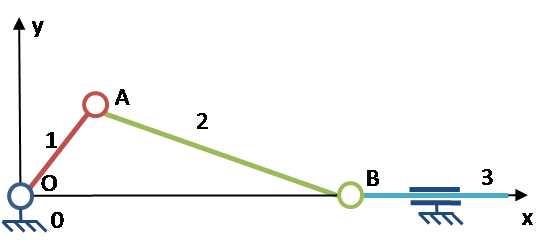
\includegraphics[width=0.7\linewidth]{img/img1}
\end{minipage}
\end{center}

En conséquence, le torseur cinématique de la liaison pivot-glissant d'axe $\overrightarrow{x}$ entre les solides 2 et 3 admet le simplification suivante : 

\begin{center}
$\left\{V_{3/0}\right\}_B=\left\{\begin{array}{cc}\omega_x & v_x \\ 0 & 0 \\ 0 & 0 \end{array} \right\}_B$ devient dans le plan $(O,\overrightarrow{x},\overrightarrow{y})$:
 \ifdef{\public}{$\left\{V_{3/0}\right\}_B=\left\{\begin{array}{cc} \sim & v_x \\ \sim & 0 \\ 0 & \sim \end{array} \right\}_B$ }{\hfill}
\end{center}

Ce type de raisonnement se généralise à tous les torseurs des liaisons et permet ainsi de minimiser le nombre d'inconnues cinématiques. Ainsi, il n'y a que 3 degrés de liberté au maximum par liaison dans \textbf{un problème plan}. 

}}


{\frame{
\frametitle{Outils de cinématique graphique}

La cinématique graphique consiste à exploiter les \textbf{propriétés} des \textbf{champs de vecteurs vitesse} par constructions \textbf{graphiques} :
\begin{itemize}
 \item \textbf{distribution de vitesse} dans un solide en rotation,
 \begin{itemize}
  \item vecteur vitesse perpendiculaire au rayon de la trajectoire,
  \item vecteur vitesse inscrit dans le triangle des vitesses.
 \end{itemize}
 \item \textbf{équiprojectivité} des vecteurs vitesses.
\end{itemize}

\vfill

Il est donc nécessaire de pouvoir représenter le mécanisme \textbf{dans un plan} qui recevra les constructions graphiques. La cinématique graphique ne peut donc s'appliquer qu'aux \textbf{mécanismes admettant une simplification plane}.
}}

{\frame{
\frametitle{Centre instantané de rotation (CIR)}

Soit un solide $S_1$ en mouvement plan par rapport à $S_0$ : 
Le torseur cinématique du mouvement de $S_1$ par rapport à $S_0$ en un point quelconque $M$ est: 

 \ifdef{\public}{
\begin{center}
$\left\{V_{S_1/S_0}\right\}_M=\left\{\begin{array}{cc} \sim & v_x \\ \sim & v_y \\ \omega_z & \sim \end{array} \right\}_M$ 
\end{center}}{\vspace{1.5cm}}

$I$ est centre instantané de rotation du solide $S_1$ par rapport à $S_0$ si :  \ifdef{\public}{
$\overrightarrow{V_{I\in S_1/S_0}}=\overrightarrow{0}$}{\hfill}

Remarques : 
\begin{itemize}
 \item $I$ est donc un point central du torseur cinématique de $S_1$ par rapport à $S_0$. Le $CIR_{(S1/S0)}$ correspond donc à l'intersection de l'axe central du torseur cinématique de $S_1/S_0$ avec le plan d'évolution du solide $S_1$,
 \item Le CIR est \og instantané \fg, c'est à dire que, dans le cas général, sa position est attachée à un instant donnée et à une position particulière du mécanisme, 
 \item Le CIR peut être un point défini en dehors de la limite matérielle du solide $S_1$. 
\end{itemize}
}}

{\frame{
\frametitle{Opérations sur le CIR}

\textbf{Répartition des vecteurs vitesse autour du CIR}

\begin{itemize}
 \item A un instant t, tout se passe comme si le solide est en rotation pure autour du CIR. 
 \begin{itemize}
  \item les vecteurs vitesses des points du solide $S_1$ sont donc orthogonaux au rayon de leur trajectoires,
  \item ils sont inscrits dans un triangle de vitesse issu du CIR.
 \end{itemize}
 \item \textit{Remarque : Si le solide $S_1$ est en liaison pivot par rapport au bâti du mécanisme, son mouvement est une rotation autour du centre de la liaison. Le CIR est alors confondu avec ce point et est fixe au cours du temps.}
\end{itemize}

\begin{minipage}{0.65\linewidth}
\textbf{Détermination graphique du CIR}

\begin{itemize}
 \item Par définition, le vecteur vitesse du point $M$ quelconque du solide $S_1$ par rapport à $S_0$ est orthogonale à la droite passant par le point $M$ et par le CIR de $S_1/S_0$. 
 \item Si on connait les directions des vitesses de deux points $M$ et $M'$ du solide $S_1$, le CIR de $S_1/S_0$  est à l'intersection des deux perpendiculaires à ces directions passant par $M$ et $M'$.
\end{itemize}
\end{minipage}
\hfill
\begin{minipage}{0.3\linewidth}
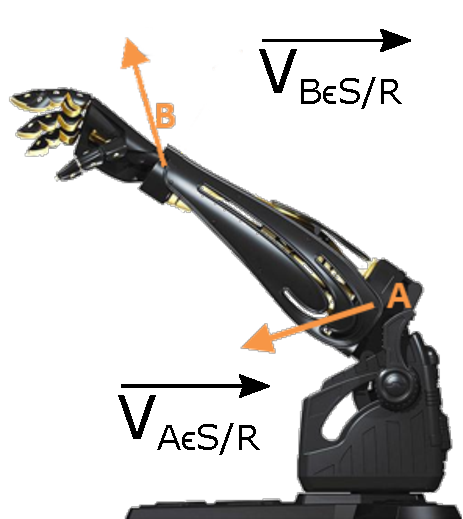
\includegraphics[width=0.9\linewidth]{img/img2}
\end{minipage}
}}


{\frame{
\frametitle{Opérations sur le CIR}

\textbf{Détermination graphique des vitesses en utilisant le CIR}

En connaissant la position de $I$, CIR de $S/R$ et la vitesse du point $A$, on détermine la vitesse d'un point $B$ quelconque du solide de la manière suivante : 

\begin{minipage}{0.7\linewidth}
 \begin{enumerate}
 \item Tracer $A'$, équidistant de $A$ $(IA=IA')$ et appartenant à $(IB)$,
 \item Tracer $\overrightarrow{V_{A'\in S_1/S_0}}$ de même norme que $\overrightarrow{V_{A\in S_1/S_0}}$ et orthogonal à $(IB)$,
 \item Tracer la droite passant par $I$ et par l'extrémité de $\overrightarrow{V_{A'\in S_1/S_0}}$, c'est le triangle des vitesses qui inscrit $\overrightarrow{V_{A\in S_1/S_0}}$,
 \item Tracer $\overrightarrow{V_{B\in S_1/S_0}}$, orthogonal à $(IB)$ et dont l'extrémité est sur la droite tracée précédemment.
 \end{enumerate}
\end{minipage}
\hfill
\begin{minipage}{0.25\linewidth}
 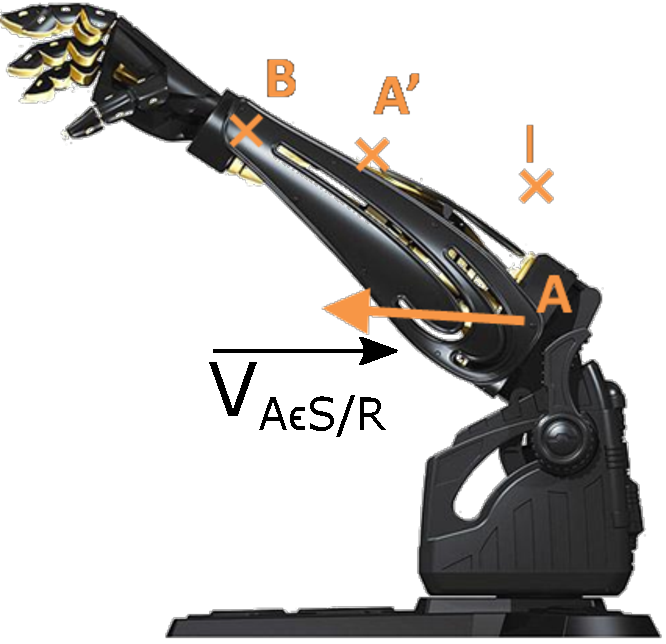
\includegraphics[width=0.9\linewidth]{img/img3}
\end{minipage}

\vfill

\textbf{Base et roulante}

\begin{itemize}
 \item La base du mouvement de $S/R$ est la trajectoire du $CIR$ de $S/R$ dans $R$, 
 \item La roulante du mouvement de $S/R$ est la trajectoire du $CIR$ de $S/R$ dans le repère lié à $S$,
 \item La base et la roulante du mouvement de $S/R$ sont à chaque instant tangentes au $CIR$ de $S/R$ et roulent sans glisser l'une sur l'autre en ce point. 
\end{itemize}
}}

{\frame{
\frametitle{Conclusion}

\begin{savoir}
Vous êtes capables :
\begin{itemize}
 \item de modéliser le comportement cinématique d'un point sans prendre en compte les liaisons,
 \item de déterminer l'accélération d'un point,
 \item de modéliser le comportement cinématique d'un point graphiquement,
 \item de tracer des champs de vecteur vitesse et accélération.
\end{itemize}
\end{savoir}

\begin{prob}
Vous devez êtes capables :
 \begin{itemize}
 \item de modéliser les actions mécaniques afin de vérifier leur influence sur le mouvement des solides.
 \end{itemize}
 Il faudra pour cela commencer par modéliser ces actions sans mouvement (statique) puis avec mouvement (dynamique).
\end{prob}
}}

\end{document}